% documentclass: article used for scientific journals, short reports, program documentation, etc
% options: fontsize 11, generate document for double sided printing, a4-paper
\documentclass[aspectratio=169]{beamer}

% package for changing page layout
% \usepackage{geometry}
% \geometry{a4paper, lmargin=40mm, rmargin=45mm, tmargin=40mm, bmargin=45mm}
% set indentation
% \setlength{\parindent}{1em}
% set factor for line spacing
% \linespread{1.0}\selectfont
% set (dynamic) additional line spacing
% \setlength{\parskip}{1ex plus 0.5ex minus 0.3ex}

% rigorous formatting (not too much hyphens)
% \fussy
% \sloppy

% package for changing page layout (used to indent whole paragraphs with adjustwidth)
\usepackage{changepage}

% input encoding for special characters (e.g. ä,ü,ö,ß), only for non english text
% options: utf8 as encoding standard, latin1
\usepackage[utf8]{inputenc}
% package for font encoding
\usepackage[T1]{fontenc}
% package for changing used language (especially for more than one language)
% options: ngerman (new spelling) or default: english
\usepackage[ngerman]{babel}
% package for times font
% \usepackage{times}
% package for latin modern fonts
\usepackage{lmodern}

% package for math symbols, functions and environments from ams(american mathematical society)
\usepackage{amsmath}
\usepackage{mathtools}
% package for extended symbols from ams
\usepackage{amssymb}
% package for math black board symbols (e.g. R,Q,Z,...)
\usepackage{bbm}
\usepackage{mathrsfs}
% package for extended symbols from stmaryrd(st mary road)
\usepackage{stmaryrd}

% pack­age im­ple­ments scal­ing of the math ex­ten­sion font cmex; used for scaling math signs
\usepackage{exscale}

% package for including extern graphics plus scaling and rotating
\usepackage{graphicx}
%package for positioning figures
\usepackage{float}
% package for changing color of font and paper
% options: using names of default colors (e.g red, black)
% \usepackage[usenames]{color}
% \usepackage[dvipsnames]{xcolor}
\definecolor{shadecolor}{gray}{0.9}
\definecolor{MidnightBlue}{rgb}{0.3, 0.3, 0.9}
\definecolor{Red}{rgb}{1, 0, 0}
\definecolor{Black}{rgb}{0, 0, 0}
% package for customising captions
\usepackage[footnotesize, hang]{caption}
% package for customising enumerations (e.g. axioms)
\usepackage{enumitem}
% calc package reimplements \setcounter, \addtocounter, \setlength and \addtolength: commands now accept an infix notation expression
\usepackage{calc}
% package for creating framed, shaded, or differently highlighted regions that can break across pages; environments: framed, oframed, shaded, shaded*, snugshade, snugshade*, leftbar, titled-frame
\usepackage{framed}
% package for creating custom "list of"
% options: titles: do not intefere with standard headings for "list of"
% \usepackage[titles]{tocloft}


% change enumeration style of equations
% \renewcommand\theequation{\thesection.\arabic{equation}}

% init list of math for definitions and theorems
% \newcommand{\listofmathcall}{Verzeichnis der Definitionen und Sätze}
% \newlistof{math}{mathlist}{\listofmathcall}
% add parentheses around argument
\newcommand{\parent}[1]{ \ifx&#1&\else (#1) \fi }
% unnumerated mathematical definition environment definiton
\newenvironment{mathdef*}[2]{
	\begin{framed}
	\noindent
	{ \fontfamily{ppl}\selectfont \textbf{\textsc{#1:}} } ~ #2 
	\par \hfill\\ 
	\fontfamily{lmr}\selectfont \itshape
}{
	\end{framed}
}
% definitions for numerated mathematical definition environment
\newcounter{mathdefc}[section]
\newcommand*{\mathdefnum}{\thesection.\arabic{mathdefc}}
\renewcommand{\themathdefc}{\mathdefnum}
\newenvironment{mathdef}[2]{
	\refstepcounter{mathdefc}
	\addcontentsline{mathlist}{figure}{\protect{\numberline{\mathdefnum}#1 ~ #2}}
	\begin{mathdef*}{#1 \mathdefnum}{#2}
}{
	\end{mathdef*}
}
% standard mathdef calls
\newcommand{\definitioncall}{Definition}
\newenvironment{stddef*}[1][]{ \begin{mathdef*}{\definitioncall}{\parent{#1}} }{ \end{mathdef*} }
\newenvironment{stddef}[1][]{ \begin{mathdef}{\definitioncall}{\parent{#1}} }{ \end{mathdef} }
% unnumerated theorem environment definition
\newenvironment{maththeorem*}[2]{
	\begin{leftbar}
	\noindent
	{ \fontfamily{ppl}\selectfont \textbf{\textsc{#1:}} } ~ #2
	\par \hfill\\ 
	\fontfamily{lmr} \fontshape{it} \selectfont
}{ 
	\end{leftbar}
}
% definitions for numerated theorem environment
\newcounter{maththeoremc}[section]
\newcommand*\maththeoremnum{\thesection.\arabic{maththeoremc}}
\renewcommand{\themaththeoremc}{\maththeoremnum}
\newenvironment{maththeorem}[2]{
	\refstepcounter{maththeoremc}
	\addcontentsline{mathlist}{figure}{\protect{\qquad\numberline{\maththeoremnum}#1 ~ #2}}
	\begin{maththeorem*}{#1 \maththeoremnum}{#2}
}{
	\end{maththeorem*}
}
% standard maththeorem calls
\newcommand{\theoremcall}{Theorem}
\newenvironment{theorem*}[1][]{ \begin{maththeorem*}{\theoremcall}{\parent{#1}} }{ \end{maththeorem*} }
\renewenvironment{theorem}[1][]{ \begin{maththeorem}{\theoremcall}{\parent{#1}} }{ \end{maththeorem} }
\newcommand{\lemmacall}{Lemma}
\newenvironment{lemma*}[1][]{ \begin{maththeorem*}{\lemmacall}{\parent{#1}} }{ \end{maththeorem*} }
\renewenvironment{lemma}[1][]{ \begin{maththeorem}{\lemmacall}{\parent{#1}} }{ \end{maththeorem} }
\newcommand{\propositioncall}{Proposition}
\newenvironment{proposition*}[1][]{ \begin{maththeorem*}{\propositioncall}{\parent{#1}} }{ \end{maththeorem*} }
\newenvironment{proposition}[1][]{ \begin{maththeorem}{\propositioncall}{\parent{#1}} }{ \end{maththeorem} }
\newcommand{\corollarycall}{Korollar}
\newenvironment{corollary*}[1][]{ \begin{maththeorem*}{\corollarycall}{\parent{#1}} }{ \end{maththeorem*} }
\renewenvironment{corollary}[1][]{ \begin{maththeorem}{\corollarycall}{\parent{#1}} }{ \end{maththeorem} }
% q.e.d. definition
\renewcommand{\qed}{ \par \hfill \fontfamily{lmr} \fontshape{it} \selectfont \mbox{q.e.d.} \\}
\newcommand{\qedbox}{ \par \hfill $\Box$ \\ }
% proof environment definition for theorems
\newenvironment{mathproof}[1]{
	\par\hfill\\
	\noindent
	{ \fontfamily{lmr}\selectfont \small \textsc{#1:}}
	\normalfont
	\small
	\begin{adjustwidth}{1em}{}
	\medskip
}{ 
	\end{adjustwidth} 
	\qedbox
}
% standard mathproof calls
\newcommand{\proofcall}{Beweis}
\renewenvironment{proof}{ \begin{mathproof}{\proofcall} }{ \end{mathproof} }
\newcommand{\proofideacall}{Beweisidee}
\newenvironment{proofidea}{ \begin{mathproof}{\proofideacall} }{ \end{mathproof} }

% new displaymath command, so that equations will not be stretched
\newcommand{\D}[1]{\mbox{$ #1 $}}
% make unnumerated equation
\newcommand{\E}[1]{\[ #1 \]}
% command for curly brackets
\newcommand{\curlb}[1]{\left\{ #1 \right\}}
% command for box brackets
\newcommand{\boxb}[1]{\left[ #1 \right]}
% command for parentheses/curved brackets
\newcommand{\curvb}[1]{\left( #1 \right)}
% command for angle brackets
\newcommand{\angleb}[1]{\left\langle #1 \right\rangle}
% command for floor brackets
\newcommand{\floorb}[1]{\left\lfloor #1 \right\rfloor}
% command for ceil brackets
\newcommand{\ceilb}[1]{\left\lceil #1 \right\rceil}
% command for creating sets
\newcommand{\set}[2]{ \left\{ #1 \enspace \middle\vert \enspace #2 \right\} }
% command for absolute value
\newcommand{\abs}[1]{\left\vert #1 \right\vert}
\newcommand{\norm}[1]{\left\| #1 \right\|}
% commands for writing limits
\newcommand{\limit}[3]{\, \longrightarrow \, #1, \ #2 \longrightarrow #3}
\newcommand{\Limit}[2]{\lim_{#1 \rightarrow #2}}
% command for differential
\newcommand{\diff}{\mathrm{d}}
\newcommand{\Diff}{\mathrm{D}}
% command for derivative
\newcommand{\Deriv}[3][]{\Diff_{#2}^{#1}#3}
\newcommand{\deriv}[3][]{\dfrac{\diff^{#1}#2(#3)}{\diff #3^{#1}}}
% command for integral
\newcommand{\integral}[4]{\int_{#1}^{#2} #3\ \diff #4}
\newcommand{\Integral}[4]{\int\limits_{#1}^{#2} #3\ \diff #4}
\newcommand{\iintegral}[2]{\int #1\ \diff #2} % indefinite integral
% mathematical definitions (standard sets)
\newcommand{\SR}{\mathds{R}} % real numbers
\newcommand{\SC}{\mathds{C}} % complex numbers
\newcommand{\SN}{\mathds{N}} % natural numbers
\newcommand{\SZ}{\mathds{Z}} % integral numbers
\newcommand{\SQ}{\mathds{Q}} % rational numbers
\newcommand{\SP}{\mathcal{P}} % power set
\newcommand{\SFP}{\mathds{P}} % polynom functions
\newcommand{\SFC}{\mathrm{C}} % complex valued functions (continous or differentiable)
\newcommand{\SFL}{\mathcal{L}} % space of integrable functions
\newcommand{\SFLL}{\mathrm{L}} % space of integrable function classes
\newcommand{\SH}{\mathcal{H}} % hilbert space
% mathematical standard functions
\DeclareMathOperator{\real}{Re} % real part
\DeclareMathOperator{\imag}{Im} % imaginary part
\newcommand{\FF}{\mathcal{F}} % fourier transform
\newcommand{\FE}{\mathbb{E}} % expectation
\DeclareMathOperator{\var}{var} % variance
\newcommand{\FN}{\mathcal{N}} % normal distribution

% command for physical units
\newcommand{\unit}[1]{\, \mathrm{#1}}

% \usepackage{calrsfs}
% \DeclareMathAlphabet{\pazocal}{OMS}{zplm}{m}{n}
\usepackage{mathrsfs}

% package for init listings(non-formatted  text) e.g. different source codes
\usepackage{listings}


% definitions for listing colors
\definecolor{codeDarkGray}{gray}{0.2}
\definecolor{codeGray}{gray}{0.4}
\definecolor{codeLightGray}{gray}{0.9}
% predefinitions for listings
\newcommand{\listingcall}{Listing}
\newlength{\listingframemargin}
\setlength{\listingframemargin}{1em}
\newlength{\listingmargin}
\setlength{\listingmargin}{0.1\textwidth}
% \newlength{\listingwidth}
% \setlength{\listingwidth}{ ( \textwidth - \listingmargin * \real{2} + \listingframemargin * \real{2} ) }
% definitions for list of listings
\newcommand{\listoflistingscall}{\listingcall -Verzeichnis}
% \newlistof{listings}{listinglist}{\listoflistingscall}
% style definition for standard code listings
\lstdefinestyle{std}{
	belowcaptionskip=0.5\baselineskip,
	breaklines=true,
	frameround=tttt,
	frame=tblr,
	xleftmargin=0em,
	xrightmargin=0em,
	showstringspaces=false,
	showtabs=false,
	% tab=\smash{\rule[-.2\baselineskip]{.4pt}{\baselineskip}\kern.5em},
	basicstyle= \fontfamily{pcr}\selectfont\footnotesize\bfseries,
	keywordstyle= \bfseries\color{MidnightBlue}, %\color{codeDarkGray},
	commentstyle= \itshape\color{codeGray},
	identifierstyle=\color{codeDarkGray},
	stringstyle=\color{BurntOrange}, %\color{codeDarkGray},
	numberstyle=\tiny\ttfamily,
	% numbers=left,
	numbersep = 2em,
	% numberstep = 5,
	% captionpos=t,
	tabsize=4,
	backgroundcolor=\color{codeLightGray},
	framexleftmargin=\listingframemargin,
	framexrightmargin=\listingframemargin
}
% definition for unnumerated listing
\newcommand{\inputlistingn}[3][]{
	\begin{center}
		\begin{adjustwidth}{\listingmargin}{\listingmargin}
			\centerline{ {\fontfamily{lmr}\selectfont\scshape \listingcall:}\quad #2 }
			\lstinputlisting[style=std, #1]{#3}
		\end{adjustwidth}
	\end{center}
}
% definition for numerated listing
\newcounter{listingc}[section]
\newcommand*\listingnum{\thesection.\arabic{listingc}}
\renewcommand{\thelistingc}{\listingnum}
\newcommand{\inputlisting}[3][]{
	\refstepcounter{listingc}
	\addcontentsline{listinglist}{figure}{\protect{\numberline{\listingnum:} #2 } }
	\inputlistingn[#1]{#2}{#3}
}


% package for including csv-tables from file
% \usepackage{csvsimple}
% package for creating, loading and manipulating databases
\usepackage{datatool}

% package for converting eps-files to pdf-files and then include them
\usepackage{epstopdf}
% use another program (ps2pdf) for converting
% !!! important: set shell_escape=1 in /etc/texmf/texmf.cnf (Linux/Ubuntu 12.04) for allowing to use other programs
% !!!			or use the command line with -shell-escape
% \epstopdfDeclareGraphicsRule{.eps}{pdf}{.pdf}{
% ps2pdf -dEPSCrop #1 \OutputFile
% }


% package for reference to last page (output number of last page)
\usepackage{lastpage}
% package for using header and footer
% options: automate terms of right and left marks
\usepackage[automark]{scrpage2}
% \setlength{\headheight}{4\baselineskip}
% set style for footer and header
% \pagestyle{scrheadings}
% \pagestyle{headings}
% clear pagestyle for redefining
% \clearscrheadfoot
% set header and footer: use <xx>head/foot[]{Text} (i...inner, o...outer, c...center, o...odd, e...even, l...left, r...right)
% \ihead[]{Fast Fourier Transform}
% \ohead[]{Markus Pawellek \\ markuspawellek@gmail.com}
% \cfoot[]{\newline\newline\newline\pagemark}
% use that for mark to last page: \pageref{LastPage}
% set header separation line
% \setheadsepline[\textwidth]{0.5pt}
% set foot separation line
% \setfootsepline[\textwidth]{0.5pt}

\usepackage{tcolorbox}
% \usepackage{tikz}
% \tcbuselibrary{listings}
\tcbuselibrary{many}

\usefonttheme[onlymath]{serif}

% package for more math blackboard symbols
\usepackage{dsfont}

% pack­age im­ple­ments scal­ing of the math ex­ten­sion font cmex; used for scaling math signs
\usepackage{exscale}

\usepackage{enumitem}
\usepackage{array}
% \usepackage{natbib}
% \bibliographystyle{plain}
\usepackage{url}

\title{Fast Fourier Transform}
\author{Markus Pawellek}
\date{03.Februar 2016}

\begin{document}
	
	\frame{\maketitle}

	\begin{frame}
		\center
		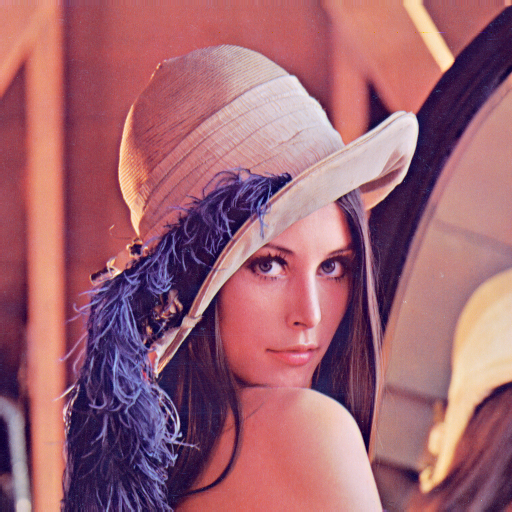
\includegraphics[scale=0.35]{example/picture-01.png}
		\hfill
		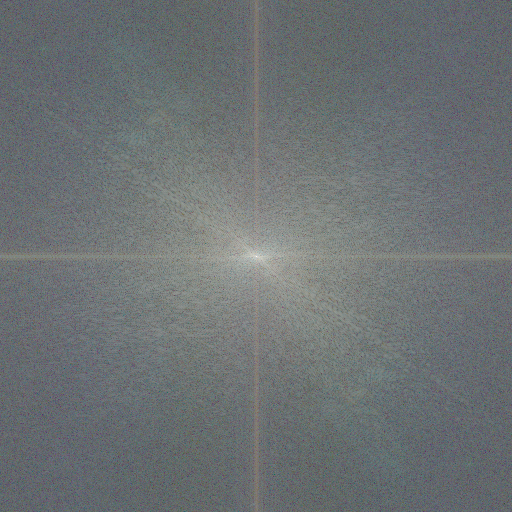
\includegraphics[scale=0.35]{example/picture-01-spec.png}
	\end{frame}

	\begin{frame}
		\center
		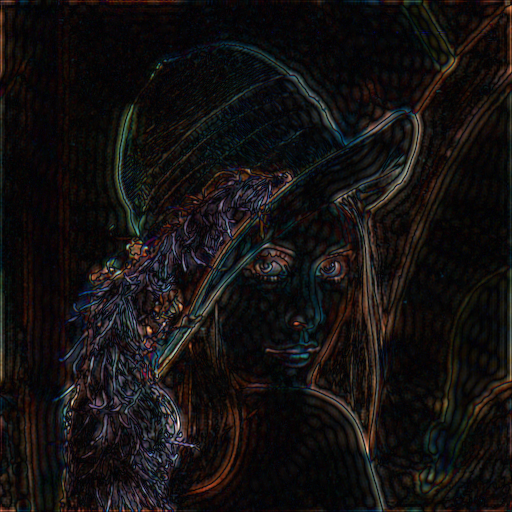
\includegraphics[scale=0.35]{example/picture-02.png}
		\hfill
		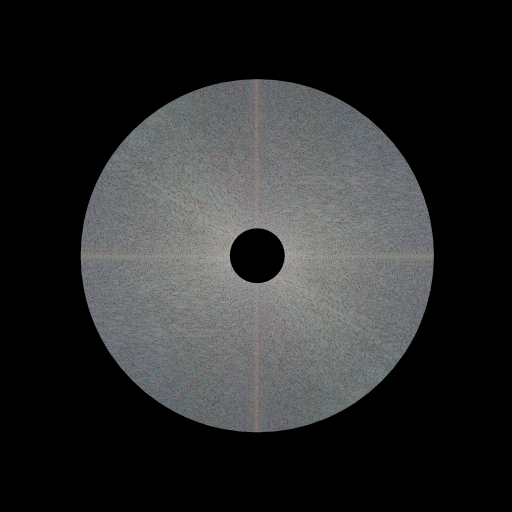
\includegraphics[scale=0.35]{example/picture-02-spec.png}
	\end{frame}

	\frame{\frametitle{Gliederung} \begin{adjustwidth}{1em}{}\tableofcontents\end{adjustwidth}}

	\section{Mathematische Grundlagen} % (fold)
	\label{sec:mathematische_grundlagen}
	
		\subsection{Fouriertransformation periodischer Funktionen} % (fold)
		\label{sub:fouriertransformation}

			\begin{frame}
				\frametitle{Fouriertransformation periodischer Funktionen}
				Um welche Funktionen geht es?\\

				\begin{enumerate}[label=(\roman*)]
					\pause\item komplexwertig: 
						\[ \tcboxmath{f:\SR\longrightarrow\SC} \]
					\pause\item periodisch mit Periode $T>0$:
						\[ \tcboxmath{\forall x\in\SR:\quad f(x) = f(x+T)} \]
					\pause\item stückweise stetig differenzierbar
				\end{enumerate}
			\end{frame}

			\begin{frame}
				\begin{tcolorbox}[title=Fouriertransformation]
					\begin{alignat*}{4}
						&\forall k\in\SZ:\quad &\FF f(k) &:= &&\ \frac{1}{T}\integral{0}{T}{ f(x)\exp\curvb{ -\frac{2\pi i}{T}kx } }{x} \\
						&\forall x\in\SR:\quad &f(x) &:= &&\ \sum_{k\in\SZ}\FF f(k)\exp\curvb{ \frac{2\pi i}{T}kx }
					\end{alignat*}
				\end{tcolorbox}
			\end{frame}

		% subsection fouriertransformation (end)

		\subsection{Diskrete Fouriertransformation} % (fold)
		\label{sub:diskrete_fouriertransformation}

			% \begin{frame}
			% 	\begin{figure}
			% 		\center
			% 		% GNUPLOT: LaTeX picture with Postscript
\begingroup
  \makeatletter
  \providecommand\color[2][]{%
    \GenericError{(gnuplot) \space\space\space\@spaces}{%
      Package color not loaded in conjunction with
      terminal option `colourtext'%
    }{See the gnuplot documentation for explanation.%
    }{Either use 'blacktext' in gnuplot or load the package
      color.sty in LaTeX.}%
    \renewcommand\color[2][]{}%
  }%
  \providecommand\includegraphics[2][]{%
    \GenericError{(gnuplot) \space\space\space\@spaces}{%
      Package graphicx or graphics not loaded%
    }{See the gnuplot documentation for explanation.%
    }{The gnuplot epslatex terminal needs graphicx.sty or graphics.sty.}%
    \renewcommand\includegraphics[2][]{}%
  }%
  \providecommand\rotatebox[2]{#2}%
  \@ifundefined{ifGPcolor}{%
    \newif\ifGPcolor
    \GPcolorfalse
  }{}%
  \@ifundefined{ifGPblacktext}{%
    \newif\ifGPblacktext
    \GPblacktexttrue
  }{}%
  % define a \g@addto@macro without @ in the name:
  \let\gplgaddtomacro\g@addto@macro
  % define empty templates for all commands taking text:
  \gdef\gplbacktext{}%
  \gdef\gplfronttext{}%
  \makeatother
  \ifGPblacktext
    % no textcolor at all
    \def\colorrgb#1{}%
    \def\colorgray#1{}%
  \else
    % gray or color?
    \ifGPcolor
      \def\colorrgb#1{\color[rgb]{#1}}%
      \def\colorgray#1{\color[gray]{#1}}%
      \expandafter\def\csname LTw\endcsname{\color{white}}%
      \expandafter\def\csname LTb\endcsname{\color{black}}%
      \expandafter\def\csname LTa\endcsname{\color{black}}%
      \expandafter\def\csname LT0\endcsname{\color[rgb]{1,0,0}}%
      \expandafter\def\csname LT1\endcsname{\color[rgb]{0,1,0}}%
      \expandafter\def\csname LT2\endcsname{\color[rgb]{0,0,1}}%
      \expandafter\def\csname LT3\endcsname{\color[rgb]{1,0,1}}%
      \expandafter\def\csname LT4\endcsname{\color[rgb]{0,1,1}}%
      \expandafter\def\csname LT5\endcsname{\color[rgb]{1,1,0}}%
      \expandafter\def\csname LT6\endcsname{\color[rgb]{0,0,0}}%
      \expandafter\def\csname LT7\endcsname{\color[rgb]{1,0.3,0}}%
      \expandafter\def\csname LT8\endcsname{\color[rgb]{0.5,0.5,0.5}}%
    \else
      % gray
      \def\colorrgb#1{\color{black}}%
      \def\colorgray#1{\color[gray]{#1}}%
      \expandafter\def\csname LTw\endcsname{\color{white}}%
      \expandafter\def\csname LTb\endcsname{\color{black}}%
      \expandafter\def\csname LTa\endcsname{\color{black}}%
      \expandafter\def\csname LT0\endcsname{\color{black}}%
      \expandafter\def\csname LT1\endcsname{\color{black}}%
      \expandafter\def\csname LT2\endcsname{\color{black}}%
      \expandafter\def\csname LT3\endcsname{\color{black}}%
      \expandafter\def\csname LT4\endcsname{\color{black}}%
      \expandafter\def\csname LT5\endcsname{\color{black}}%
      \expandafter\def\csname LT6\endcsname{\color{black}}%
      \expandafter\def\csname LT7\endcsname{\color{black}}%
      \expandafter\def\csname LT8\endcsname{\color{black}}%
    \fi
  \fi
  \setlength{\unitlength}{0.0500bp}%
  \begin{picture}(6802.00,3968.00)%
    \gplgaddtomacro\gplbacktext{%
      \csname LTb\endcsname%
      \put(682,704){\makebox(0,0)[r]{\strut{}-2}}%
      \put(682,2204){\makebox(0,0)[r]{\strut{} 0}}%
      \put(682,3703){\makebox(0,0)[r]{\strut{} 2}}%
      \put(814,484){\makebox(0,0){\strut{} 0}}%
      \put(1746,484){\makebox(0,0){\strut{} 1}}%
      \put(2678,484){\makebox(0,0){\strut{} 2}}%
      \put(3610,484){\makebox(0,0){\strut{} 3}}%
      \put(4541,484){\makebox(0,0){\strut{} 4}}%
      \put(5473,484){\makebox(0,0){\strut{} 5}}%
      \put(6405,484){\makebox(0,0){\strut{} 6}}%
      \put(176,2203){\rotatebox{-270}{\makebox(0,0){\strut{}$y$}}}%
      \put(3609,154){\makebox(0,0){\strut{}$x$}}%
    }%
    \gplgaddtomacro\gplfronttext{%
      \csname LTb\endcsname%
      \put(5418,1207){\makebox(0,0)[r]{\strut{}Funktion}}%
      \csname LTb\endcsname%
      \put(5418,987){\makebox(0,0)[r]{\strut{}Stützpunkte}}%
    }%
    \gplbacktext
    \put(0,0){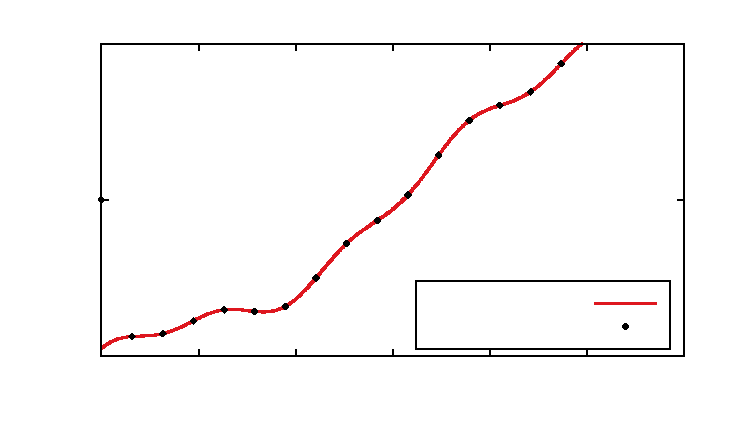
\includegraphics{example-beamer}}%
    \gplfronttext
  \end{picture}%
\endgroup

			% 	\end{figure}
			% \end{frame}

			\begin{frame}
				\frametitle{Diskrete Fouriertransformation}
				% \frametitle{Orthonormalbasis}
				\begin{tcolorbox}[title=Orthonormalbasis des $\SC^n$ bezüglich Standardskalarprodukt]
					\[ D := \set{\omega_k:\mathrm{N}_n\longrightarrow\SC}{ k\in\mathrm{N}_n,\ \forall x\in\mathrm{N}_n:\ \omega_k(x) = \exp\curvb{\frac{2\pi i}{n}kx} } \]
				\end{tcolorbox}
				\begin{tcolorbox}[title=Parsevalsche Gleichung]
					\[ \forall x\in\mathrm{N}_n: \ g(x) = \sum_{k=0}^{n-1} \angleb{\omega_k, g} \omega_k(x) \]
				\end{tcolorbox}
			\end{frame}

			\begin{frame}[label=dft]
				\begin{tcolorbox}[title=Diskrete Fouriertransformation]
					\begin{alignat*}{4}
						&\forall k\in\mathrm{N}_n: \ &&\ \hat{g}(k) := \frac{1}{n} &&\sum_{x=0}^{n-1} g(x)\exp\curvb{ -\frac{2\pi i}{n}kx } \\
						&\forall x\in\mathrm{N}_n: \ &&\ g(x) := &&\sum_{k=0}^{n-1} \hat{g}(k)\exp\curvb{ \frac{2\pi i}{n}xk }
					\end{alignat*}
				\end{tcolorbox}
			\end{frame}

			\begin{frame}
				\frametitle{Ein Beispiel}
				\begin{tcolorbox}
					\[ g:\curlb{0,1,2,3,4}\longrightarrow\SC,\qquad g(x)=x \]
					\begin{table}
						\center
						\setlength{\extrarowheight}{4pt}
						\begin{tabular}{c|c}
							\hline
							$x$ & $\sim\hat{g}(x)$ \\ [1ex]
							\hline
							\hline
							$0$ & $10$ \\
							$1$ & $-0.5 + 0.688191\,i$ \\
							$2$ & $-0.5 + 0.162460\,i$ \\
							$3$ & $-0.5 - 0.162460\,i$ \\
							$4$ & $-0.5 - 0.688191\,i$ \\
							\hline
						\end{tabular}
						\caption{Fourierkoeffizienten der Beispielfunktion $g$}
						\label{tab:example}
					\end{table}
				\end{tcolorbox}
			\end{frame}

			\begin{frame}
			\frametitle{Ein Beispiel}
				\begin{figure}
					\center
					% GNUPLOT: LaTeX picture with Postscript
\begingroup
  \makeatletter
  \providecommand\color[2][]{%
    \GenericError{(gnuplot) \space\space\space\@spaces}{%
      Package color not loaded in conjunction with
      terminal option `colourtext'%
    }{See the gnuplot documentation for explanation.%
    }{Either use 'blacktext' in gnuplot or load the package
      color.sty in LaTeX.}%
    \renewcommand\color[2][]{}%
  }%
  \providecommand\includegraphics[2][]{%
    \GenericError{(gnuplot) \space\space\space\@spaces}{%
      Package graphicx or graphics not loaded%
    }{See the gnuplot documentation for explanation.%
    }{The gnuplot epslatex terminal needs graphicx.sty or graphics.sty.}%
    \renewcommand\includegraphics[2][]{}%
  }%
  \providecommand\rotatebox[2]{#2}%
  \@ifundefined{ifGPcolor}{%
    \newif\ifGPcolor
    \GPcolorfalse
  }{}%
  \@ifundefined{ifGPblacktext}{%
    \newif\ifGPblacktext
    \GPblacktexttrue
  }{}%
  % define a \g@addto@macro without @ in the name:
  \let\gplgaddtomacro\g@addto@macro
  % define empty templates for all commands taking text:
  \gdef\gplbacktext{}%
  \gdef\gplfronttext{}%
  \makeatother
  \ifGPblacktext
    % no textcolor at all
    \def\colorrgb#1{}%
    \def\colorgray#1{}%
  \else
    % gray or color?
    \ifGPcolor
      \def\colorrgb#1{\color[rgb]{#1}}%
      \def\colorgray#1{\color[gray]{#1}}%
      \expandafter\def\csname LTw\endcsname{\color{white}}%
      \expandafter\def\csname LTb\endcsname{\color{black}}%
      \expandafter\def\csname LTa\endcsname{\color{black}}%
      \expandafter\def\csname LT0\endcsname{\color[rgb]{1,0,0}}%
      \expandafter\def\csname LT1\endcsname{\color[rgb]{0,1,0}}%
      \expandafter\def\csname LT2\endcsname{\color[rgb]{0,0,1}}%
      \expandafter\def\csname LT3\endcsname{\color[rgb]{1,0,1}}%
      \expandafter\def\csname LT4\endcsname{\color[rgb]{0,1,1}}%
      \expandafter\def\csname LT5\endcsname{\color[rgb]{1,1,0}}%
      \expandafter\def\csname LT6\endcsname{\color[rgb]{0,0,0}}%
      \expandafter\def\csname LT7\endcsname{\color[rgb]{1,0.3,0}}%
      \expandafter\def\csname LT8\endcsname{\color[rgb]{0.5,0.5,0.5}}%
    \else
      % gray
      \def\colorrgb#1{\color{black}}%
      \def\colorgray#1{\color[gray]{#1}}%
      \expandafter\def\csname LTw\endcsname{\color{white}}%
      \expandafter\def\csname LTb\endcsname{\color{black}}%
      \expandafter\def\csname LTa\endcsname{\color{black}}%
      \expandafter\def\csname LT0\endcsname{\color{black}}%
      \expandafter\def\csname LT1\endcsname{\color{black}}%
      \expandafter\def\csname LT2\endcsname{\color{black}}%
      \expandafter\def\csname LT3\endcsname{\color{black}}%
      \expandafter\def\csname LT4\endcsname{\color{black}}%
      \expandafter\def\csname LT5\endcsname{\color{black}}%
      \expandafter\def\csname LT6\endcsname{\color{black}}%
      \expandafter\def\csname LT7\endcsname{\color{black}}%
      \expandafter\def\csname LT8\endcsname{\color{black}}%
    \fi
  \fi
  \setlength{\unitlength}{0.0500bp}%
  \begin{picture}(6802.00,3968.00)%
    \gplgaddtomacro\gplbacktext{%
      \csname LTb\endcsname%
      \put(682,1079){\makebox(0,0)[r]{\strut{} 0}}%
      \put(682,1829){\makebox(0,0)[r]{\strut{} 2}}%
      \put(682,2578){\makebox(0,0)[r]{\strut{} 4}}%
      \put(682,3328){\makebox(0,0)[r]{\strut{} 6}}%
      \put(814,484){\makebox(0,0){\strut{}-1}}%
      \put(1613,484){\makebox(0,0){\strut{} 0}}%
      \put(2411,484){\makebox(0,0){\strut{} 1}}%
      \put(3210,484){\makebox(0,0){\strut{} 2}}%
      \put(4009,484){\makebox(0,0){\strut{} 3}}%
      \put(4808,484){\makebox(0,0){\strut{} 4}}%
      \put(5606,484){\makebox(0,0){\strut{} 5}}%
      \put(6405,484){\makebox(0,0){\strut{} 6}}%
      \put(176,2203){\rotatebox{-270}{\makebox(0,0){\strut{}$y$}}}%
      \put(3609,154){\makebox(0,0){\strut{}$x$}}%
    }%
    \gplgaddtomacro\gplfronttext{%
      \csname LTb\endcsname%
      \put(5418,3420){\makebox(0,0)[r]{\strut{}trigonometrisches Polynom $p_5$}}%
      \csname LTb\endcsname%
      \put(5418,3200){\makebox(0,0)[r]{\strut{}Stützpunkte von $g$}}%
    }%
    \gplbacktext
    \put(0,0){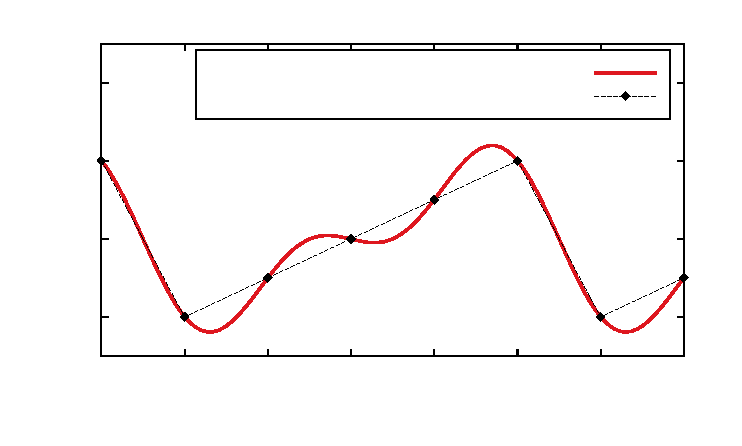
\includegraphics{example-2}}%
    \gplfronttext
  \end{picture}%
\endgroup

				\end{figure}
			\end{frame}
		
		% subsection diskrete_fouriertransformation (end)

	% section mathematische_grundlagen (end)

	\section{Serieller Algorithmus} % (fold)
	\label{sec:serieller_algorithmus}
	
		\subsection{Idee der Fast Fourier Transform} % (fold)
		\label{sub:idee_der_fast_fourier_transform}

			\againframe{dft}

			\begin{frame}
				\frametitle{Idee der Fast Fourier Transform}
				\begin{tcolorbox}[title=Rekursionsformeln der DFT]
					\begin{alignat*}{3}
						g_0:\mathrm{N}_m\longrightarrow\SC,\qquad g_0(x) &:=&& \ g(2x) \\
						g_1:\mathrm{N}_m\longrightarrow\SC,\qquad g_1(x) &:=&& \ g(2x+1)
					\end{alignat*}
					\begin{alignat*}{5}
						&\FF_n g(k) &&=&& \ \frac{1}{2}\curvb{\FF_m g_0(k) + e^{-\frac{\pi i}{m}k} \ \FF_m g_1(k)} \\
						&\FF_n g(k+m) &&=&& \ \frac{1}{2}\curvb{\FF_m g_0(k) - e^{-\frac{\pi i}{m}k} \ \FF_m g_1(k)}
					\end{alignat*}
				\end{tcolorbox}
			\end{frame}

		% subsection idee_der_fast_fourier_transform (end)

		\subsection{Rekursiver Algorithmus} % (fold)
		\label{sub:rekursiver_algorithmus}

			\begin{frame}
				\frametitle{Ein rekursiver Algorithmus}
				\begin{tcolorbox}[breakable, colframe=black,colbacktitle=white,coltitle=black,enhanced, titlerule=0.1pt, boxrule=0.5pt, attach boxed title to top center={yshift=-2mm},enhanced, arc=5pt,title=Listing:\quad rekursiver FFT-Algorithmus Teil 1]
					\scriptsize
					\begin{tabbing}
	\quad\=\quad\=\quad\=\kill
	$\mathbf{program} \textrm{ Recursive-FFT}$\\
	$\mathbf{declare}$\\
		\>$\mathbf{procedure} \textrm{ fft}(\mathit{out},\mathit{in}\ :\ \mathrm{array}[0..2^{q}-1-1] \textrm{ of complex}\ ;\ q\ :\ \mathrm{integer});$ \\
		\>$t\ :\ \textrm{integer}\ ;$\\
		\>$\omega,b,c\ :\ \mathrm{array}[0..2^{p}-1] \textrm{ of complex}$\\
	$\mathbf{initially}$\\
		\>$\color{MidnightBlue}\curlb{\textit{\ttfamily look-up table for twiddle factors}}$\\
		\>$\langle \ ;\ t\ :\ 0\leq t<2^p\ ::\ \omega[t] = \exp(-\frac{2\pi it}{n})\ \rangle\ ;$\\
		\>$\langle \ ;\ t\ :\ 0\leq t<2^p\ ::\ b[t] = g(t)\ \rangle$\\
	$\mathbf{assign}$\\
		\>$\mathrm{fft}(c,b,p)$\\
	$\mathbf{end}$\\
\end{tabbing}
				\end{tcolorbox}
			\end{frame}

			\begin{frame}
				\frametitle{Ein rekursiver Algorithmus}
				\begin{tcolorbox}[breakable, colframe=black,colbacktitle=white,coltitle=black,enhanced, titlerule=0.1pt, boxrule=0.5pt, attach boxed title to top center={yshift=-2mm},enhanced, arc=5pt,title=Listing:\quad rekursiver FFT-Algorithmus Teil 2]
					\scriptsize
					\begin{tabbing}
	\quad\=\quad\=\quad\=\kill
	$\color{MidnightBlue}\curlb{\textit{\ttfamily extra procedure for recursive algorithm}}$\\
	$\mathbf{procedure} \textrm{ fft}(\mathit{out},\mathit{in}\ :\ \mathrm{array}[0..2^{q}-1-1] \textrm{ of complex}\ ;\ q\ :\ \mathrm{integer})$ \\
	$\mathbf{begin}$\\
		\>$\mathbf{if}\ q=0\ \mathbf{then}$\\
			\>\>$\mathit{out}[0] = \mathit{in}[0]$\\
		\>$\mathbf{else}\ \mathbf{begin}$\\
		% \>$$\\
			\>\>$\mathrm{fft}(\mathit{out}[0..2^{q-1}-1]\ ,\ \mathit{in}[0..2..2^{q}-2]\ ,\ q-1);$\\
			\>\>$\mathrm{fft}(\mathit{out}[2^{q-1}..2^q-1]\ ,\ \mathit{in}[1..2..2^{q}-1]\ ,\ q-1);$\\
			% \\
			\>\>$\langle \ \|\ t\ :\ 0\leq t<2^{q-1}\ ::$\\
				\>\>\>$\boxb{ \begin{array}{l} b[t] \\ b[t+2^{q-1}] \end{array} } := \dfrac{1}{2} \boxb{ \begin{array}{lr} 1 & \omega[2^{p-q}t] \\ 1 & -\omega[2^{p-q}t] \end{array} }\boxb{ \begin{array}{l} b[t] \\ b[t+2^{q-1}] \end{array} }$\\
			\>\>$\rangle$\\
		\>$\mathbf{end}$\\
	$\mathbf{end}$\\
\end{tabbing}
				\end{tcolorbox}
			\end{frame}
		
		% subsection rekursiver_algorithmus (end)

		\subsection{Von Bit-Reversal zu Butterfly} % (fold)
		\label{sub:von_bit_reversal_zu_butterfly}

			\begin{frame}
				\frametitle{Bit-Reversal}
				\begin{figure}
					\center
					\scriptsize
					\unitlength0.8cm
\begin{picture}(9,9)(-1,-3)
	\put(-0.1,5){$b_0$}
	\put(0.9,5){$b_1$}
	\put(1.9,5){$b_2$}
	\put(2.9,5){$b_3$}
	\put(3.9,5){$b_4$}
	\put(4.9,5){$b_5$}
	\put(5.9,5){$b_6$}
	\put(6.9,5){$b_7$}

	\put(-0.1,3){$b_0$}
	\put(0.9,3){$b_2$}
	\put(1.9,3){$b_4$}
	\put(2.9,3){$b_6$}
	\put(3.9,3){$b_1$}
	\put(4.9,3){$b_3$}
	\put(5.9,3){$b_5$}
	\put(6.9,3){$b_7$}

	\put(-0.1,1){$b_0$}
	\put(0.9,1){$b_4$}
	\put(1.9,1){$b_2$}
	\put(2.9,1){$b_6$}
	\put(3.9,1){$b_1$}
	\put(4.9,1){$b_5$}
	\put(5.9,1){$b_3$}
	\put(6.9,1){$b_7$}

	\put(-0.1,-1){$b_0$}
	\put(0.9,-1){$b_4$}
	\put(1.9,-1){$b_2$}
	\put(2.9,-1){$b_6$}
	\put(3.9,-1){$b_1$}
	\put(4.9,-1){$b_5$}
	\put(5.9,-1){$b_3$}
	\put(6.9,-1){$b_7$}

	\put(-0.1,-2.4){$\tilde{b}_0$}
	\put(0.9,-2.4){$\tilde{b}_1$}
	\put(1.9,-2.4){$\tilde{b}_2$}
	\put(2.9,-2.4){$\tilde{b}_3$}
	\put(3.9,-2.4){$\tilde{b}_4$}
	\put(4.9,-2.4){$\tilde{b}_5$}
	\put(5.9,-2.4){$\tilde{b}_6$}
	\put(6.9,-2.4){$\tilde{b}_7$}

	\put(-0.1,-1.8){\rotatebox{90}{$:=$}}
	\put(0.9,-1.8){\rotatebox{90}{$:=$}}
	\put(1.9,-1.8){\rotatebox{90}{$:=$}}
	\put(2.9,-1.8){\rotatebox{90}{$:=$}}
	\put(3.9,-1.8){\rotatebox{90}{$:=$}}
	\put(4.9,-1.8){\rotatebox{90}{$:=$}}
	\put(5.9,-1.8){\rotatebox{90}{$:=$}}
	\put(6.9,-1.8){\rotatebox{90}{$:=$}}

	\put(0,4.6){\vector(0,-1){1}}
	\put(1,4.6){\vector(3,-1){3}}
	\put(2,4.6){\vector(-1,-1){1}}
	\put(3,4.6){\vector(2,-1){2}}
	\put(4,4.6){\vector(-2,-1){2}}
	\put(5,4.6){\vector(1,-1){1}}
	\put(6,4.6){\vector(-3,-1){3}}
	\put(7,4.6){\vector(0,-1){1}}

	\put(0,2.6){\vector(0,-1){1}}
	\put(1,2.6){\vector(1,-1){1}}
	\put(2,2.6){\vector(-1,-1){1}}
	\put(3,2.6){\vector(0,-1){1}}
	\put(4,2.6){\vector(0,-1){1}}
	\put(5,2.6){\vector(1,-1){1}}
	\put(6,2.6){\vector(-1,-1){1}}
	\put(7,2.6){\vector(0,-1){1}}

	\put(0,0.6){\vector(0,-1){1}}
	\put(1,0.6){\vector(0,-1){1}}
	\put(2,0.6){\vector(0,-1){1}}
	\put(3,0.6){\vector(0,-1){1}}
	\put(4,0.6){\vector(0,-1){1}}
	\put(5,0.6){\vector(0,-1){1}}
	\put(6,0.6){\vector(0,-1){1}}
	\put(7,0.6){\vector(0,-1){1}}

	\put(-0.3,4.7){\dashbox{0.1}(7.6,0.8)}

	\put(-0.3,2.7){\dashbox{0.1}(3.6,0.8)}
	\put(3.7,2.7){\dashbox{0.1}(3.6,0.8)}

	\put(-0.3,0.7){\dashbox{0.1}(1.6,0.8)}
	\put(1.7,0.7){\dashbox{0.1}(1.6,0.8)}
	\put(3.7,0.7){\dashbox{0.1}(1.6,0.8)}
	\put(5.7,0.7){\dashbox{0.1}(1.6,0.8)}

	\put(-0.3,-1.3){\dashbox{0.1}(0.6,0.8)}
	\put(0.7,-1.3){\dashbox{0.1}(0.6,0.8)}
	\put(1.7,-1.3){\dashbox{0.1}(0.6,0.8)}
	\put(2.7,-1.3){\dashbox{0.1}(0.6,0.8)}
	\put(3.7,-1.3){\dashbox{0.1}(0.6,0.8)}
	\put(4.7,-1.3){\dashbox{0.1}(0.6,0.8)}
	\put(5.7,-1.3){\dashbox{0.1}(0.6,0.8)}
	\put(6.7,-1.3){\dashbox{0.1}(0.6,0.8)}

	\put(-0.3,-2.7){\dashbox{0.1}(7.6,0.8)}
\end{picture}
				\end{figure}
			\end{frame}

			\begin{frame}
				\frametitle{Butterfly Graph}
				\begin{figure}
					\center
					% \scriptsize
					\unitlength1cm
\begin{picture}(9,8)(-1,-2)
	\put(-0.1,5){$c_0$}
	\put(0.9,5){$c_1$}
	\put(1.9,5){$c_2$}
	\put(2.9,5){$c_3$}
	\put(3.9,5){$c_4$}
	\put(4.9,5){$c_5$}
	\put(5.9,5){$c_6$}
	\put(6.9,5){$c_7$}

	\put(-0.1,3){$c_0$}
	\put(0.9,3){$c_1$}
	\put(1.9,3){$c_2$}
	\put(2.9,3){$c_3$}
	\put(3.9,3){$c_4$}
	\put(4.9,3){$c_5$}
	\put(5.9,3){$c_6$}
	\put(6.9,3){$c_7$}

	\put(-0.1,3.15){$^+$}
	\put(0.9,3.15){$^-$}
	\put(1.9,3.15){$^+$}
	\put(2.9,3.15){$^-$}
	\put(3.9,3.15){$^+$}
	\put(4.9,3.15){$^-$}
	\put(5.9,3.15){$^+$}
	\put(6.9,3.15){$^-$}

	\put(-0.1,1){$c_0$}
	\put(0.9,1){$c_1$}
	\put(1.9,1){$c_2$}
	\put(2.9,1){$c_3$}
	\put(3.9,1){$c_4$}
	\put(4.9,1){$c_5$}
	\put(5.9,1){$c_6$}
	\put(6.9,1){$c_7$}

	\put(-0.1,1.15){$^+$}
	\put(0.9,1.15){$^+$}
	\put(1.9,1.15){$^-$}
	\put(2.9,1.15){$^-$}
	\put(3.9,1.15){$^+$}
	\put(4.9,1.15){$^+$}
	\put(5.9,1.15){$^-$}
	\put(6.9,1.15){$^-$}

	\put(-0.1,-1){$c_0$}
	\put(0.9,-1){$c_1$}
	\put(1.9,-1){$c_2$}
	\put(2.9,-1){$c_3$}
	\put(3.9,-1){$c_4$}
	\put(4.9,-1){$c_5$}
	\put(5.9,-1){$c_6$}
	\put(6.9,-1){$c_7$}

	\put(-0.1,-0.85){$^+$}
	\put(0.9,-0.85){$^+$}
	\put(1.9,-0.85){$^+$}
	\put(2.9,-0.85){$^+$}
	\put(3.9,-0.85){$^-$}
	\put(4.9,-0.85){$^-$}
	\put(5.9,-0.85){$^-$}
	\put(6.9,-0.85){$^-$}

	% \put(-0.1,-2.4){$\tilde{b}_0$}
	% \put(0.9,-2.4){$\tilde{b}_1$}
	% \put(1.9,-2.4){$\tilde{b}_2$}
	% \put(2.9,-2.4){$\tilde{b}_3$}
	% \put(3.9,-2.4){$\tilde{b}_4$}
	% \put(4.9,-2.4){$\tilde{b}_5$}
	% \put(5.9,-2.4){$\tilde{b}_6$}
	% \put(6.9,-2.4){$\tilde{b}_7$}

	% \put(-0.1,-1.8){\rotatebox{90}{$:=$}}
	% \put(0.9,-1.8){\rotatebox{90}{$:=$}}
	% \put(1.9,-1.8){\rotatebox{90}{$:=$}}
	% \put(2.9,-1.8){\rotatebox{90}{$:=$}}
	% \put(3.9,-1.8){\rotatebox{90}{$:=$}}
	% \put(4.9,-1.8){\rotatebox{90}{$:=$}}
	% \put(5.9,-1.8){\rotatebox{90}{$:=$}}
	% \put(6.9,-1.8){\rotatebox{90}{$:=$}}

	\put(0,4.6){\vector(0,-1){1}}
	\put(1,4.6){\vector(0,-1){1}}
	\put(2,4.6){\vector(0,-1){1}}
	\put(3,4.6){\vector(0,-1){1}}
	\put(4,4.6){\vector(0,-1){1}}
	\put(5,4.6){\vector(0,-1){1}}
	\put(6,4.6){\vector(0,-1){1}}
	\put(7,4.6){\vector(0,-1){1}}

	\put(0,4.6){\vector(1,-1){1}}
	\put(2,4.6){\vector(1,-1){1}}
	\put(4,4.6){\vector(1,-1){1}}
	\put(6,4.6){\vector(1,-1){1}}
	\put(1,4.6){\vector(-1,-1){1}}
	\put(3,4.6){\vector(-1,-1){1}}
	\put(5,4.6){\vector(-1,-1){1}}
	\put(7,4.6){\vector(-1,-1){1}}

	\put(0,2.6){\vector(0,-1){1}}
	\put(1,2.6){\vector(0,-1){1}}
	\put(2,2.6){\vector(0,-1){1}}
	\put(3,2.6){\vector(0,-1){1}}
	\put(4,2.6){\vector(0,-1){1}}
	\put(5,2.6){\vector(0,-1){1}}
	\put(6,2.6){\vector(0,-1){1}}
	\put(7,2.6){\vector(0,-1){1}}

	\put(0,2.6){\vector(2,-1){2}}
	\put(1,2.6){\vector(2,-1){2}}
	\put(4,2.6){\vector(2,-1){2}}
	\put(5,2.6){\vector(2,-1){2}}
	\put(2,2.6){\vector(-2,-1){2}}
	\put(3,2.6){\vector(-2,-1){2}}
	\put(6,2.6){\vector(-2,-1){2}}
	\put(7,2.6){\vector(-2,-1){2}}

	\put(0,0.6){\vector(0,-1){1}}
	\put(1,0.6){\vector(0,-1){1}}
	\put(2,0.6){\vector(0,-1){1}}
	\put(3,0.6){\vector(0,-1){1}}
	\put(4,0.6){\vector(0,-1){1}}
	\put(5,0.6){\vector(0,-1){1}}
	\put(6,0.6){\vector(0,-1){1}}
	\put(7,0.6){\vector(0,-1){1}}

	\put(0,0.6){\vector(4,-1){4}}
	\put(1,0.6){\vector(4,-1){4}}
	\put(2,0.6){\vector(4,-1){4}}
	\put(3,0.6){\vector(4,-1){4}}
	\put(4,0.6){\vector(-4,-1){4}}
	\put(5,0.6){\vector(-4,-1){4}}
	\put(6,0.6){\vector(-4,-1){4}}
	\put(7,0.6){\vector(-4,-1){4}}


	% \put(0,4.6){\vector(0,-1){1}}
	% \put(1,4.6){\vector(3,-1){3}}
	% \put(2,4.6){\vector(-1,-1){1}}
	% \put(3,4.6){\vector(2,-1){2}}
	% \put(4,4.6){\vector(-2,-1){2}}
	% \put(5,4.6){\vector(1,-1){1}}
	% \put(6,4.6){\vector(-3,-1){3}}
	% \put(7,4.6){\vector(0,-1){1}}

	% \put(0,2.6){\vector(0,-1){1}}
	% \put(1,2.6){\vector(1,-1){1}}
	% \put(2,2.6){\vector(-1,-1){1}}
	% \put(3,2.6){\vector(0,-1){1}}
	% \put(4,2.6){\vector(0,-1){1}}
	% \put(5,2.6){\vector(1,-1){1}}
	% \put(6,2.6){\vector(-1,-1){1}}
	% \put(7,2.6){\vector(0,-1){1}}

	

	\put(-0.3,-1.3){\dashbox{0.1}(7.6,0.8)}

	\put(-0.3,0.7){\dashbox{0.1}(3.6,0.8)}
	\put(3.7,0.7){\dashbox{0.1}(3.6,0.8)}

	\put(-0.3,2.7){\dashbox{0.1}(1.6,0.8)}
	\put(1.7,2.7){\dashbox{0.1}(1.6,0.8)}
	\put(3.7,2.7){\dashbox{0.1}(1.6,0.8)}
	\put(5.7,2.7){\dashbox{0.1}(1.6,0.8)}

	\put(-0.3,4.7){\dashbox{0.1}(0.6,0.8)}
	\put(0.7,4.7){\dashbox{0.1}(0.6,0.8)}
	\put(1.7,4.7){\dashbox{0.1}(0.6,0.8)}
	\put(2.7,4.7){\dashbox{0.1}(0.6,0.8)}
	\put(3.7,4.7){\dashbox{0.1}(0.6,0.8)}
	\put(4.7,4.7){\dashbox{0.1}(0.6,0.8)}
	\put(5.7,4.7){\dashbox{0.1}(0.6,0.8)}
	\put(6.7,4.7){\dashbox{0.1}(0.6,0.8)}

	% \put(-0.3,-2.7){\dashbox{0.1}(7.6,0.8)}
\end{picture}
				\end{figure}
			\end{frame}
		
		% subsection von_bit_reversal_zu_butterfly (end)

		\subsection{Nicht-Rekursiver Algorithmus} % (fold)
		\label{sub:nicht_rekursiver_algorithmus}

			\begin{frame}
				\frametitle{Nicht-Rekursiver Algorithmus}
				\begin{tcolorbox}[breakable, colframe=black,colbacktitle=white,coltitle=black,enhanced, titlerule=0.1pt, boxrule=0.5pt, attach boxed title to top center={yshift=-2mm},enhanced, arc=5pt,title=Listing:\quad nicht-rekursiver FFT-Algorithmus]
					\scriptsize
					\begin{tabbing}
	\quad\=\quad\=\quad\=\kill
	$\mathbf{program} \textrm{ Serial-FFT}$\\
	$\mathbf{declare}$\\
		% \>$\mathbf{procedure} \textrm{ fft}(\mathit{out},\mathit{in}\ :\ \mathrm{array}[0..2^{q}-1-1] \textrm{ of complex}\ ;\ q\ :\ \mathrm{integer});$ \\
		\>$m,t\ :\ \textrm{integer}\ ;$\\
		\>$\omega,b\ :\ \mathrm{array}[0..2^{p}-1] \textrm{ of complex}$\\
	$\mathbf{initially}$\\
		\>$\color{MidnightBlue}\curlb{\textit{\ttfamily look-up table for twiddle factors}}$\\
		\>$\langle \ ;\ t\ :\ 0\leq t<2^p\ ::\ \omega[t] = \exp(-\frac{2\pi it}{n})\ \rangle\ ;$\\
		\>$\color{MidnightBlue}\curlb{\textit{\ttfamily bit-reverse ordering}}$\\
		\>$\langle \ ;\ t\ :\ 0\leq t<2^p\ ::\ b[t] = g(\sigma_p(t))\ \rangle$\\
	$\mathbf{assign}$\\
		% \>$\mathrm{fft}(c,b,p)$\\
		\>$\color{MidnightBlue}\curlb{\textit{\ttfamily butterfly calculation}}$\\
		\>$\langle \ ;\ m\ :\ 0\leq m<p\ ::$\\
			\>\>$\langle \ \|\ t\ :\ 0\leq t<2^{p}-1\ \mathbf{and}\ t\wedge 2^m=0\ ::$\\
				\>\>\>$\boxb{ \begin{array}{l} b[t] \\ b[t+2^m] \end{array} } := \dfrac{1}{2} \boxb{ \begin{array}{lr} 1 & \omega[2^{p-m-1}t\ \mathrm{mod}\ 2^{p-1}] \\ 1 & -\omega[2^{p-m-1}t\ \mathrm{mod}\ 2^{p-1}] \end{array} }\boxb{ \begin{array}{l} b[t] \\ b[t+2^m] \end{array} }$\\
			\>\>$\rangle$\\
		\>$\rangle$\\
	$\mathbf{end}$\\
	% \\
	% \\
	% $\mathbf{procedure} \textrm{ fft}(\mathit{out},\mathit{in}\ :\ \mathrm{array}[0..2^{q}-1-1] \textrm{ of complex}\ ;\ q\ :\ \mathrm{integer})$ \\
	% $\mathbf{begin}$\\
	% 	\>$\mathbf{if}\ q=0\ \mathbf{then}$\\
	% 		\>\>$\mathit{out}[0] = \mathit{in}[0]$\\
	% 	\>$\mathbf{else}$\\
	% 	\>$\mathbf{begin}$\\
	% 		\>\>$\mathrm{fft}(\mathit{out}[0..2^{q-1}-1]\ ,\ \mathit{in}[0..2..2^{q}-2]\ ,\ q-1);$\\
	% 		\>\>$\mathrm{fft}(\mathit{out}[2^{q-1}..2^q-1]\ ,\ \mathit{in}[1..2..2^{q}-1]\ ,\ q-1);$\\
	% 		\\
	% 		\>\>$\langle \ \|\ t\ :\ 0\leq t<2^{q-1}\ ::$\\
	% 			\>\>\>$\boxb{ \begin{array}{l} b[t] \\ b[t+2^{q-1}] \end{array} } := \dfrac{1}{2} \boxb{ \begin{array}{lr} 1 & \omega[2^{p-q}t] \\ 1 & -\omega[2^{p-q}t] \end{array} }\boxb{ \begin{array}{l} b[t] \\ b[t+2^{q-1}] \end{array} }$\\
	% 		\>\>$\rangle$\\
	% 	\>$\mathbf{end}$\\
	% $\mathbf{end}$\\
\end{tabbing}
				\end{tcolorbox}
			\end{frame}
		
		% subsection nicht_rekursiver_algorithmus (end)

	% section serieller_algorithmus (end)

	\section{Parallelisierung} % (fold)
	\label{sec:parallelisierung}
	
		\subsection{Verteilung der Daten} % (fold)
		\label{sub:verteilung_der_daten}

			\begin{frame}
				\frametitle{Datenverteilung}
				\begin{figure}[h]
					\center
					\unitlength1cm
\begin{picture}(9,2)(-1,0)
	\put(-0.1,1){$\tilde{b}_0$}
	\put(0.9,1){$\tilde{b}_1$}
	\put(1.9,1){$\tilde{b}_2$}
	\put(2.9,1){$\tilde{b}_3$}
	\put(3.9,1){$\tilde{b}_4$}
	\put(4.9,1){$\tilde{b}_5$}
	\put(5.9,1){$\tilde{b}_6$}
	\put(6.9,1){$\tilde{b}_7$}

	\put(-0.3,0.7){\framebox(1.6,0.8)}
	\put(1.7,0.7){\framebox(1.6,0.8)}
	\put(3.7,0.7){\framebox(1.6,0.8)}
	\put(5.7,0.7){\framebox(1.6,0.8)}

	\put(0.4,0.3){$\rho_0$}
	\put(2.4,0.3){$\rho_1$}
	\put(4.4,0.3){$\rho_2$}
	\put(6.4,0.3){$\rho_3$}
\end{picture}
					\caption{Verteilung des Eingabearrays $\tilde{b}$ auf den Prozessen $\rho_i$ für $p=3,q=2$}
					\label{fig:data-distribution}
				\end{figure}
			\end{frame}
		
		% subsection verteilung_der_daten (end)

		\subsection{Kommunikation} % (fold)
		\label{sub:kommunikation}

			\begin{frame}
				\frametitle{Kommunikation}
				\begin{figure}[h]
					\center
					\unitlength1cm
\begin{picture}(9,8)(-1,-2)
	\put(-0.1,5){$b_0$}
	\put(0.9,5){$b_1$}
	\put(1.9,5){$b_2$}
	\put(2.9,5){$b_3$}
	\put(3.9,5){$b_4$}
	\put(4.9,5){$b_5$}
	\put(5.9,5){$b_6$}
	\put(6.9,5){$b_7$}

	\put(-0.1,3){$b_0$}
	\put(0.9,3){$b_1$}
	\put(1.9,3){$b_2$}
	\put(2.9,3){$b_3$}
	\put(3.9,3){$b_4$}
	\put(4.9,3){$b_5$}
	\put(5.9,3){$b_6$}
	\put(6.9,3){$b_7$}

	\put(-0.1,3.15){$^+$}
	\put(0.9,3.15){$^-$}
	\put(1.9,3.15){$^+$}
	\put(2.9,3.15){$^-$}
	\put(3.9,3.15){$^+$}
	\put(4.9,3.15){$^-$}
	\put(5.9,3.15){$^+$}
	\put(6.9,3.15){$^-$}

	\put(-0.1,1){$b_0$}
	\put(0.9,1){$b_1$}
	\put(1.9,1){$b_2$}
	\put(2.9,1){$b_3$}
	\put(3.9,1){$b_4$}
	\put(4.9,1){$b_5$}
	\put(5.9,1){$b_6$}
	\put(6.9,1){$b_7$}

	\put(-0.1,1.15){$^+$}
	\put(0.9,1.15){$^+$}
	\put(1.9,1.15){$^-$}
	\put(2.9,1.15){$^-$}
	\put(3.9,1.15){$^+$}
	\put(4.9,1.15){$^+$}
	\put(5.9,1.15){$^-$}
	\put(6.9,1.15){$^-$}

	\put(-0.1,-1){$b_0$}
	\put(0.9,-1){$b_1$}
	\put(1.9,-1){$b_2$}
	\put(2.9,-1){$b_3$}
	\put(3.9,-1){$b_4$}
	\put(4.9,-1){$b_5$}
	\put(5.9,-1){$b_6$}
	\put(6.9,-1){$b_7$}

	\put(-0.1,-0.85){$^+$}
	\put(0.9,-0.85){$^+$}
	\put(1.9,-0.85){$^+$}
	\put(2.9,-0.85){$^+$}
	\put(3.9,-0.85){$^-$}
	\put(4.9,-0.85){$^-$}
	\put(5.9,-0.85){$^-$}
	\put(6.9,-0.85){$^-$}

	% \put(-0.1,-2.4){$\tilde{b}_0$}
	% \put(0.9,-2.4){$\tilde{b}_1$}
	% \put(1.9,-2.4){$\tilde{b}_2$}
	% \put(2.9,-2.4){$\tilde{b}_3$}
	% \put(3.9,-2.4){$\tilde{b}_4$}
	% \put(4.9,-2.4){$\tilde{b}_5$}
	% \put(5.9,-2.4){$\tilde{b}_6$}
	% \put(6.9,-2.4){$\tilde{b}_7$}

	% \put(-0.1,-1.8){\rotatebox{90}{$:=$}}
	% \put(0.9,-1.8){\rotatebox{90}{$:=$}}
	% \put(1.9,-1.8){\rotatebox{90}{$:=$}}
	% \put(2.9,-1.8){\rotatebox{90}{$:=$}}
	% \put(3.9,-1.8){\rotatebox{90}{$:=$}}
	% \put(4.9,-1.8){\rotatebox{90}{$:=$}}
	% \put(5.9,-1.8){\rotatebox{90}{$:=$}}
	% \put(6.9,-1.8){\rotatebox{90}{$:=$}}

	\put(0,4.6){\vector(0,-1){1}}
	\put(1,4.6){\vector(0,-1){1}}
	\put(2,4.6){\vector(0,-1){1}}
	\put(3,4.6){\vector(0,-1){1}}
	\put(4,4.6){\vector(0,-1){1}}
	\put(5,4.6){\vector(0,-1){1}}
	\put(6,4.6){\vector(0,-1){1}}
	\put(7,4.6){\vector(0,-1){1}}

	\put(0,4.6){\vector(1,-1){1}}
	\put(2,4.6){\vector(1,-1){1}}
	\put(4,4.6){\vector(1,-1){1}}
	\put(6,4.6){\vector(1,-1){1}}
	\put(1,4.6){\vector(-1,-1){1}}
	\put(3,4.6){\vector(-1,-1){1}}
	\put(5,4.6){\vector(-1,-1){1}}
	\put(7,4.6){\vector(-1,-1){1}}

	\put(0,2.6){\vector(0,-1){1}}
	\put(1,2.6){\vector(0,-1){1}}
	\put(2,2.6){\vector(0,-1){1}}
	\put(3,2.6){\vector(0,-1){1}}
	\put(4,2.6){\vector(0,-1){1}}
	\put(5,2.6){\vector(0,-1){1}}
	\put(6,2.6){\vector(0,-1){1}}
	\put(7,2.6){\vector(0,-1){1}}

	\put(0,2.6){\vector(2,-1){2}}
	\put(1,2.6){\vector(2,-1){2}}
	\put(4,2.6){\vector(2,-1){2}}
	\put(5,2.6){\vector(2,-1){2}}
	\put(2,2.6){\vector(-2,-1){2}}
	\put(3,2.6){\vector(-2,-1){2}}
	\put(6,2.6){\vector(-2,-1){2}}
	\put(7,2.6){\vector(-2,-1){2}}

	\put(0,0.6){\vector(0,-1){1}}
	\put(1,0.6){\vector(0,-1){1}}
	\put(2,0.6){\vector(0,-1){1}}
	\put(3,0.6){\vector(0,-1){1}}
	\put(4,0.6){\vector(0,-1){1}}
	\put(5,0.6){\vector(0,-1){1}}
	\put(6,0.6){\vector(0,-1){1}}
	\put(7,0.6){\vector(0,-1){1}}

	\put(0,0.6){\vector(4,-1){4}}
	\put(1,0.6){\vector(4,-1){4}}
	\put(2,0.6){\vector(4,-1){4}}
	\put(3,0.6){\vector(4,-1){4}}
	\put(4,0.6){\vector(-4,-1){4}}
	\put(5,0.6){\vector(-4,-1){4}}
	\put(6,0.6){\vector(-4,-1){4}}
	\put(7,0.6){\vector(-4,-1){4}}


	% \put(0,4.6){\vector(0,-1){1}}
	% \put(1,4.6){\vector(3,-1){3}}
	% \put(2,4.6){\vector(-1,-1){1}}
	% \put(3,4.6){\vector(2,-1){2}}
	% \put(4,4.6){\vector(-2,-1){2}}
	% \put(5,4.6){\vector(1,-1){1}}
	% \put(6,4.6){\vector(-3,-1){3}}
	% \put(7,4.6){\vector(0,-1){1}}

	% \put(0,2.6){\vector(0,-1){1}}
	% \put(1,2.6){\vector(1,-1){1}}
	% \put(2,2.6){\vector(-1,-1){1}}
	% \put(3,2.6){\vector(0,-1){1}}
	% \put(4,2.6){\vector(0,-1){1}}
	% \put(5,2.6){\vector(1,-1){1}}
	% \put(6,2.6){\vector(-1,-1){1}}
	% \put(7,2.6){\vector(0,-1){1}}

	\color{Red}
	% \linethickness{0.3mm}
	\thicklines

	\put(-0.4,-1.4){\dashbox{0.2}(7.8,1)}

	\put(-0.4,0.6){\dashbox{0.2}(3.8,1)}
	\put(3.6,0.6){\dashbox{0.2}(3.8,1)}

	\put(-0.4,2.6){\dashbox{0.2}(1.8,1)}
	\put(1.6,2.6){\dashbox{0.2}(1.8,1)}
	\put(3.6,2.6){\dashbox{0.2}(1.8,1)}
	\put(5.6,2.6){\dashbox{0.2}(1.8,1)}

	\put(-0.4,4.6){\dashbox{0.2}(0.8,1)}
	\put(0.6,4.6){\dashbox{0.2}(0.8,1)}
	\put(1.6,4.6){\dashbox{0.2}(0.8,1)}
	\put(2.6,4.6){\dashbox{0.2}(0.8,1)}
	\put(3.6,4.6){\dashbox{0.2}(0.8,1)}
	\put(4.6,4.6){\dashbox{0.2}(0.8,1)}
	\put(5.6,4.6){\dashbox{0.2}(0.8,1)}
	\put(6.6,4.6){\dashbox{0.2}(0.8,1)}


	\color{Black}
	\thinlines
	% \linethickness{0.3mm}

	\put(-0.3,4.7){\framebox(1.6,0.8)}
	\put(1.7,4.7){\framebox(1.6,0.8)}
	\put(3.7,4.7){\framebox(1.6,0.8)}
	\put(5.7,4.7){\framebox(1.6,0.8)}

	\put(-0.3,2.7){\framebox(1.6,0.8)}
	\put(1.7,2.7){\framebox(1.6,0.8)}
	\put(3.7,2.7){\framebox(1.6,0.8)}
	\put(5.7,2.7){\framebox(1.6,0.8)}

	\put(-0.3,0.7){\framebox(1.6,0.8)}
	\put(1.7,0.7){\framebox(1.6,0.8)}
	\put(3.7,0.7){\framebox(1.6,0.8)}
	\put(5.7,0.7){\framebox(1.6,0.8)}

	\put(-0.3,-1.3){\framebox(1.6,0.8)}
	\put(1.7,-1.3){\framebox(1.6,0.8)}
	\put(3.7,-1.3){\framebox(1.6,0.8)}
	\put(5.7,-1.3){\framebox(1.6,0.8)}

	% \put(-0.3,-2.7){\dashbox{0.1}(7.6,0.8)}
\end{picture}
					\caption{Funktionsweise eines Butterfly Graph auf mehreren Prozessen am Beispiel von $p=3,q=2$}
					\label{fig:butterfly-parallel}
				\end{figure}
			\end{frame}
		
		% subsection kommunikation (end)

		\subsection{Paralleler Algorithmus} % (fold)
		\label{sub:paralleler_algorithmus}

			\begin{frame}
				\frametitle{Ein paralleler Algorithmus}
				\begin{tcolorbox}[breakable, colframe=black,colbacktitle=white,coltitle=black,enhanced, titlerule=0.1pt, boxrule=0.5pt, attach boxed title to top center={yshift=-2mm},enhanced, arc=5pt,title=Listing:\quad paralleler FFT-Algorithmus Teil 1]
					\scriptsize
					\begin{tabbing}
	\quad\=\quad\=\quad\=\quad\=\kill
	$0..2^q-1\ \|\ \rho\ \mathbf{program} \textrm{ Parallel-FFT}$\\
	$\mathbf{declare}$\\
		% \>$\mathbf{procedure} \textrm{ fft}(\mathit{out},\mathit{in}\ :\ \mathrm{array}[0..2^{q}-1-1] \textrm{ of complex}\ ;\ q\ :\ \mathrm{integer});$ \\
		\>$m,t\ :\ \textrm{integer}\ ;$\\
		\>$\omega\ :\ \mathrm{array}[0..2^{p}-1] \textrm{ of complex}\ ;$\\
		\>$b,x\ :\ \mathrm{array}[0..2^{p-q}-1] \textrm{ of complex}$\\
	$\mathbf{initially}$\\
		\>$\color{MidnightBlue}\curlb{\textit{\ttfamily look-up table for twiddle factors}}$\\
		\>$\langle \ ;\ t\ :\ 0\leq t<2^p\ ::\ \omega[t] = \exp(-\frac{2\pi it}{n})\ \rangle\ ;$\\
		\>$\color{MidnightBlue}\curlb{\textit{\ttfamily bit-reverse ordering}}$\\
		\>$\langle \ ;\ t\ :\ 0\leq t<2^{p-q}\ ::\ b[t] = g(\sigma_p(2^{p-q}\rho + t))\ \rangle$\\
	$\mathbf{assign}$\\
		% \>$\mathrm{fft}(c,b,p)$\\
		\>$\color{MidnightBlue}\curlb{\textit{\ttfamily butterfly calculation with no communication}}$\\
		\>$\langle \ ;\ m\ :\ 0\leq m<p-q\ ::$\\
			\>\>$\langle \ ;\ t\ :\ 0\leq t<2^{p-q}\ \mathbf{and}\ t\wedge 2^m=0\ ::$\\
				\>\>\>$\boxb{ \begin{array}{l} b[t] \\ b[t+2^m] \end{array} } := \dfrac{1}{2} \boxb{ \begin{array}{lr} 1 & \omega[\xi(m,\rho, t)] \\ 1 & -\omega[\xi(m,\rho, t)] \end{array} }\boxb{ \begin{array}{l} b[t] \\ b[t+2^m] \end{array} }$\\
			\>\>$\rangle$\\
		\>$\rangle\ ;$\\
\end{tabbing}
				\end{tcolorbox}
			\end{frame}

			\begin{frame}
				\frametitle{Ein paralleler Algorithmus}
				\begin{tcolorbox}[breakable, colframe=black,colbacktitle=white,coltitle=black,enhanced, titlerule=0.1pt, boxrule=0.5pt, attach boxed title to top center={yshift=-2mm},enhanced, arc=5pt,title=Listing:\quad paralleler FFT-Algorithmus Teil 2]
					\scriptsize
					\begin{tabbing}
	\quad\=\quad\=\quad\=\quad\=\kill
		\>$\color{MidnightBlue}\curlb{\textit{\ttfamily butterfly calculation with communication}}$\\
		\>$\langle \ ;\ m\ :\ 0\leq m<q\ ::$\\
			\>\>$\mathbf{send}\ \set{b[t]}{0\leq t<2^{p-q}}\ \mathbf{to}\ \rho\bar{\vee}2^m\ ;$\\
			\>\>$\mathbf{receive}\ \set{x[t]}{0\leq t<2^{p-q}}\ \mathbf{from}\ \rho\bar{\vee}2^m\ ;$\\
			% \>\>$\langle \ ;\ t\ :\ 0\leq t<2^{p-q}-1\ \mathbf{and}\ t\wedge 2^m=0\ ::$\\
			\>\>$\mathbf{if}\ \rho\wedge 2^m=0\ \mathbf{then}$\\
				\>\>\>$\langle \ ;\ t\ :\ 0\leq t<2^{p-q}\ \mathbf{and}\ t\wedge 2^m=0\ ::$\\
					\>\>\>\>$b[t]:=\frac{1}{2}\curvb{b[t] + \omega[\xi(m,\rho, t)]x[t]}\ \rangle$\\
			\>\>$\mathbf{else}$\\
				\>\>\>$\langle \ ;\ t\ :\ 0\leq t<2^{p-q}\ \mathbf{and}\ t\wedge 2^m=0\ ::$\\
					\>\>\>\>$b[t]:=\frac{1}{2}\curvb{x[t] - \omega[\xi(m,\rho, t)]b[t]}\ \rangle$\\
			\>\>$\mathbf{end}$\\
			% \>\>$\rangle$\\
		\>$\rangle$\\
	$\mathbf{end}$\\
\end{tabbing}
				\end{tcolorbox}
			\end{frame}
		
		% subsection paralleler_algorithmus (end)

		\subsection{Leistungsanalyse} % (fold)
		\label{sub:leistungsanalyse}

			\begin{frame}
				\frametitle{Leistungsanalyse}
				\begin{tcolorbox}[title=Gesamtzeit des parallelen FFT-Algorithmus]
					\[ T(n,P) = 2\frac{n}{P}\curvb{ \tau_\mathrm{A}\log_2 n + \beta\log_2 P } + 2\tau_\mathrm{S}\log_2 P  \]
				\end{tcolorbox}

				\begin{tcolorbox}[title=Speedup des parallelen FFT-Algorithmus]
					\[ S(n,P):=\frac{T(n,1)}{T(n,P)} = \frac{P}{ 1 + \frac{\log_2 P}{\log_2 n}\curvb{ \frac{\beta}{\tau_\mathrm{A}} + \frac{P}{n}\frac{\tau_{\mathrm{S}}}{\tau_{\mathrm{A}}} } } \]
				\end{tcolorbox}
			\end{frame}
		
		% subsection leistungsanalyse (end)

	% section parallelisierung (end)

	\section{Literatur und Quellen} % (fold)
	\label{sec:literatur_und_quellen}

		\begin{frame}
			\frametitle{Literatur und Quellen}
			\begin{enumerate}[label = {[\arabic*]}]
				\item \url{http://www.ejectamenta.com/Imaging-Experiments/fourierimagefiltering.html}
				\item \url{https://en.wikipedia.org/wiki/Fast_Fourier_transform}
				\item \url{https://en.wikipedia.org/wiki/Cooley-Tukey_FFT_algorithm}
				\item \url{http://cnx.org/contents/ulXtQbN7@15/Implementing-FFTs-in-Practice}
				\item Eric F. Van de Velde, \textit{Concurrent Scientific Computing}, Springer-Verlag, 1994
				\item Rami Shakarchi, Elias M. Stein, \textit{Fourier Analysis - An Introduction}, Band I der \textit{Princeton Lectures in Analysis}, Princeton University Press, 2003
				\item Jürgen Elstrodt, \textit{Maß- und Integrationstheorie}, Springer, 2009
				\item Martin Hermann, \textit{Numerische Mathematik}, Oldenbourg Verlag München, 2011
			\end{enumerate}
		\end{frame}

	
	% section literatur_und_quellen (end)

	% \begin{frame}
	% 	% \inputlisting{test}{code-1.txt}
	% 		\footnotesize
	% 	\begin{tcolorbox}[breakable, colframe=black,colbacktitle=white,coltitle=black, attach boxed title to top center={yshift=-2mm},enhanced, titlerule=0.1pt, boxrule=0.5pt, arc=5pt,title=Listing:\quad paralleler FFT-Algorithmus]
	% 		\begin{tabbing}
	\quad\=\quad\=\quad\=\quad\=\kill
	$0..2^q-1\ \|\ \rho\ \mathbf{program} \textrm{ Parallel-FFT}$\\
	$\mathbf{declare}$\\
		% \>$\mathbf{procedure} \textrm{ fft}(\mathit{out},\mathit{in}\ :\ \mathrm{array}[0..2^{q}-1-1] \textrm{ of complex}\ ;\ q\ :\ \mathrm{integer});$ \\
		\>$m,t\ :\ \textrm{integer}\ ;$\\
		\>$\omega\ :\ \mathrm{array}[0..2^{p}-1] \textrm{ of complex}\ ;$\\
		\>$b,x\ :\ \mathrm{array}[0..2^{p-q}-1] \textrm{ of complex}$\\
	$\mathbf{initially}$\\
		\>$\color{MidnightBlue}\curlb{\textit{\ttfamily look-up table for twiddle factors}}$\\
		\>$\langle \ ;\ t\ :\ 0\leq t<2^p\ ::\ \omega[t] = \exp(-\frac{2\pi it}{n})\ \rangle\ ;$\\
		\>$\color{MidnightBlue}\curlb{\textit{\ttfamily bit-reverse ordering}}$\\
		\>$\langle \ ;\ t\ :\ 0\leq t<2^{p-q}\ ::\ b[t] = g(\sigma_p(2^{p-q}\rho + t))\ \rangle$\\
	$\mathbf{assign}$\\
		% \>$\mathrm{fft}(c,b,p)$\\
		\>$\color{MidnightBlue}\curlb{\textit{\ttfamily butterfly calculation with no communication}}$\\
		\>$\langle \ ;\ m\ :\ 0\leq m<p-q\ ::$\\
			\>\>$\langle \ ;\ t\ :\ 0\leq t<2^{p-q}\ \mathbf{and}\ t\wedge 2^m=0\ ::$\\
				\>\>\>$\boxb{ \begin{array}{l} b[t] \\ b[t+2^m] \end{array} } := \dfrac{1}{2} \boxb{ \begin{array}{lr} 1 & \omega[\xi(m,\rho, t)] \\ 1 & -\omega[\xi(m,\rho, t)] \end{array} }\boxb{ \begin{array}{l} b[t] \\ b[t+2^m] \end{array} }$\\
			\>\>$\rangle$\\
		\>$\rangle\ ;$\\
		\>$\color{MidnightBlue}\curlb{\textit{\ttfamily butterfly calculation with communication}}$\\
		\>$\langle \ ;\ m\ :\ 0\leq m<q\ ::$\\
			\>\>$\mathbf{send}\ \set{b[t]}{0\leq t<2^{p-q}}\ \mathbf{to}\ \rho\bar{\vee}2^m\ ;$\\
			\>\>$\mathbf{receive}\ \set{x[t]}{0\leq t<2^{p-q}}\ \mathbf{from}\ \rho\bar{\vee}2^m\ ;$\\
			% \>\>$\langle \ ;\ t\ :\ 0\leq t<2^{p-q}-1\ \mathbf{and}\ t\wedge 2^m=0\ ::$\\
			\>\>$\mathbf{if}\ \rho\wedge 2^m=0\ \mathbf{then}$\\
				\>\>\>$\langle \ ;\ t\ :\ 0\leq t<2^{p-q}\ \mathbf{and}\ t\wedge 2^m=0\ ::$\\
					\>\>\>\>$b[t]:=\frac{1}{2}\curvb{b[t] + \omega[\xi(m,\rho, t)]x[t]}\ \rangle$\\
			\>\>$\mathbf{else}$\\
				\>\>\>$\langle \ ;\ t\ :\ 0\leq t<2^{p-q}\ \mathbf{and}\ t\wedge 2^m=0\ ::$\\
					\>\>\>\>$b[t]:=\frac{1}{2}\curvb{x[t] - \omega[\xi(m,\rho, t)]b[t]}\ \rangle$\\
			\>\>$\mathbf{end}$\\
			% \>\>$\rangle$\\
		\>$\rangle$\\
	$\mathbf{end}$\\
\end{tabbing}
	% 	\end{tcolorbox}
	% \end{frame}

	% \begin{frame}
	% \begin{figure}
	% 		% GNUPLOT: LaTeX picture with Postscript
\begingroup
  \makeatletter
  \providecommand\color[2][]{%
    \GenericError{(gnuplot) \space\space\space\@spaces}{%
      Package color not loaded in conjunction with
      terminal option `colourtext'%
    }{See the gnuplot documentation for explanation.%
    }{Either use 'blacktext' in gnuplot or load the package
      color.sty in LaTeX.}%
    \renewcommand\color[2][]{}%
  }%
  \providecommand\includegraphics[2][]{%
    \GenericError{(gnuplot) \space\space\space\@spaces}{%
      Package graphicx or graphics not loaded%
    }{See the gnuplot documentation for explanation.%
    }{The gnuplot epslatex terminal needs graphicx.sty or graphics.sty.}%
    \renewcommand\includegraphics[2][]{}%
  }%
  \providecommand\rotatebox[2]{#2}%
  \@ifundefined{ifGPcolor}{%
    \newif\ifGPcolor
    \GPcolorfalse
  }{}%
  \@ifundefined{ifGPblacktext}{%
    \newif\ifGPblacktext
    \GPblacktexttrue
  }{}%
  % define a \g@addto@macro without @ in the name:
  \let\gplgaddtomacro\g@addto@macro
  % define empty templates for all commands taking text:
  \gdef\gplbacktext{}%
  \gdef\gplfronttext{}%
  \makeatother
  \ifGPblacktext
    % no textcolor at all
    \def\colorrgb#1{}%
    \def\colorgray#1{}%
  \else
    % gray or color?
    \ifGPcolor
      \def\colorrgb#1{\color[rgb]{#1}}%
      \def\colorgray#1{\color[gray]{#1}}%
      \expandafter\def\csname LTw\endcsname{\color{white}}%
      \expandafter\def\csname LTb\endcsname{\color{black}}%
      \expandafter\def\csname LTa\endcsname{\color{black}}%
      \expandafter\def\csname LT0\endcsname{\color[rgb]{1,0,0}}%
      \expandafter\def\csname LT1\endcsname{\color[rgb]{0,1,0}}%
      \expandafter\def\csname LT2\endcsname{\color[rgb]{0,0,1}}%
      \expandafter\def\csname LT3\endcsname{\color[rgb]{1,0,1}}%
      \expandafter\def\csname LT4\endcsname{\color[rgb]{0,1,1}}%
      \expandafter\def\csname LT5\endcsname{\color[rgb]{1,1,0}}%
      \expandafter\def\csname LT6\endcsname{\color[rgb]{0,0,0}}%
      \expandafter\def\csname LT7\endcsname{\color[rgb]{1,0.3,0}}%
      \expandafter\def\csname LT8\endcsname{\color[rgb]{0.5,0.5,0.5}}%
    \else
      % gray
      \def\colorrgb#1{\color{black}}%
      \def\colorgray#1{\color[gray]{#1}}%
      \expandafter\def\csname LTw\endcsname{\color{white}}%
      \expandafter\def\csname LTb\endcsname{\color{black}}%
      \expandafter\def\csname LTa\endcsname{\color{black}}%
      \expandafter\def\csname LT0\endcsname{\color{black}}%
      \expandafter\def\csname LT1\endcsname{\color{black}}%
      \expandafter\def\csname LT2\endcsname{\color{black}}%
      \expandafter\def\csname LT3\endcsname{\color{black}}%
      \expandafter\def\csname LT4\endcsname{\color{black}}%
      \expandafter\def\csname LT5\endcsname{\color{black}}%
      \expandafter\def\csname LT6\endcsname{\color{black}}%
      \expandafter\def\csname LT7\endcsname{\color{black}}%
      \expandafter\def\csname LT8\endcsname{\color{black}}%
    \fi
  \fi
  \setlength{\unitlength}{0.0500bp}%
  \begin{picture}(6802.00,3968.00)%
    \gplgaddtomacro\gplbacktext{%
      \csname LTb\endcsname%
      \put(682,1079){\makebox(0,0)[r]{\strut{} 0}}%
      \put(682,1829){\makebox(0,0)[r]{\strut{} 2}}%
      \put(682,2578){\makebox(0,0)[r]{\strut{} 4}}%
      \put(682,3328){\makebox(0,0)[r]{\strut{} 6}}%
      \put(814,484){\makebox(0,0){\strut{}-1}}%
      \put(1613,484){\makebox(0,0){\strut{} 0}}%
      \put(2411,484){\makebox(0,0){\strut{} 1}}%
      \put(3210,484){\makebox(0,0){\strut{} 2}}%
      \put(4009,484){\makebox(0,0){\strut{} 3}}%
      \put(4808,484){\makebox(0,0){\strut{} 4}}%
      \put(5606,484){\makebox(0,0){\strut{} 5}}%
      \put(6405,484){\makebox(0,0){\strut{} 6}}%
      \put(176,2203){\rotatebox{-270}{\makebox(0,0){\strut{}$y$}}}%
      \put(3609,154){\makebox(0,0){\strut{}$x$}}%
    }%
    \gplgaddtomacro\gplfronttext{%
      \csname LTb\endcsname%
      \put(5418,3420){\makebox(0,0)[r]{\strut{}trigonometrisches Polynom $p_5$}}%
      \csname LTb\endcsname%
      \put(5418,3200){\makebox(0,0)[r]{\strut{}Stützpunkte von $g$}}%
    }%
    \gplbacktext
    \put(0,0){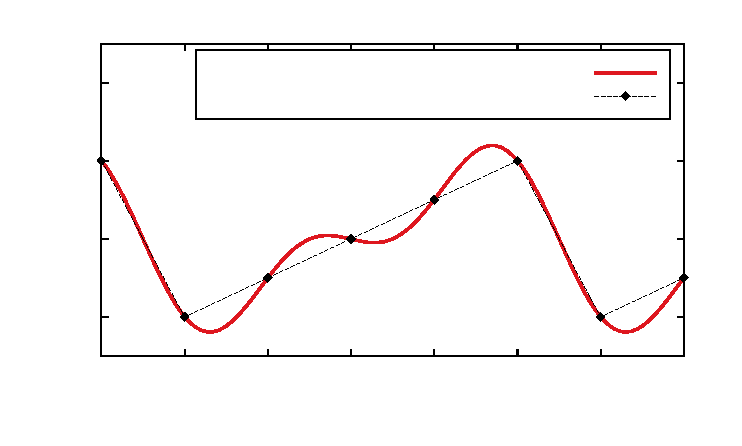
\includegraphics{example-2}}%
    \gplfronttext
  \end{picture}%
\endgroup

	% 		% \caption{Interpolation}
	% 	\end{figure}
	% \end{frame}

\end{document}